%!TEX root = informe.tex

\IEEEPARstart{F}{i}nalizada la enumeraci\'on de ciertos rubros que motiven la investigaci\'on sobre el tema, con la adici\'on de una breve explicaci\'on del problema a trabajar y de la justificación teórica detrás del método de interpolación, nos dedicaremos a desarrollar con mayor precisi\'on cada m\'etodo n\'umerico en cuesti\'on. Recordemos que estos métodos intentan atacar el problema de construir, a partir de un video filmado en tiempo real, nuevos frames que den la sensaci\'on de que el video original ha sido ralentizado (efecto de \emph{slowmotion}), o, aún mejor, filmado con una cámara de alta frecuencia.

\subsection{Aclaraciones \'utiles para la comprensi\'on del desarrollo}

Antes de ingresar al campo que abarca la explicaci\'on de los m\'etodos, queremos esclarecer ciertas frases o palabras claves que ocupar\'an terreno en el resto de la secci\'on:

\begin{itemize}
	\item \textit{Frame original}: Se le dar\'a nombre al cuadro que pertenece al video original, es decir, aquel archivo que no contiene los frames agregados que conciben al efecto de c\'amara lenta.
	\item \textit{Frame artificial}: Lo llamaremos a aquellos cuadros que se realizar\'an a partir del procedimiento que dicho m\'etodo vaya planeando. En esta ocasi\'on, se puede ratificar que los mismos se crearan en conjunto, y entre medio de un par de frames originales.
	\item \textit{Cantidad de frames a adjuntar}: Nos referiremos al par\'ametro que decide cu\'antos cuadros artificiales le adicionaremos entre cada par de frames originales. Lo denotaremos con las letras $fr$.
	\item \textit{Matriz frame}: Aunque no se hablar\'a de ese nombre en particular, es fundamental aclarar que en cualquier comentario acerca de los valores o p\'ixeles de un frame, se lo est\'a especificando como una matriz de $m$ x $n$ (visto como la resoluci\'on del video) que lleva los valores del $0$ al $255$, inclusive (escala de grises).
	\item \textit{P\'ixel}: Transladamos esta palabra asociada a la im\'agen digital al campo del \'algebra lineal. Por lo tanto, se lo considerar\'a como un componente de la matriz frame cuyos valores estan restringido en el rango $[0;255]$.
\end{itemize}

\subsection{Los m\'etodos propuestos}

Para la explicación de todos los métodos consideramos dado (como parámetros del problema) el video sobre el cual trabajar y la cantidad $fr$ de frames a generar entre cada par de frames del original. Llamaremos \emph{frames artificiales} a los frames generados por los métodos, y \emph{frames originales} a los frames provenientes del video original.

\subsubsection{Cuadro m\'as cercano}

Este m\'etodo se basa en una idea de car\'acter simplista, muy sencilla de implementar, y que nos permitirá tener una base para establecer comparaciones con métodos más inteligentes. A pesar de esto, puede resultar precisa para ciertos tipos de videos, como por ejemplo, la filmaci\'on de un objeto inmóvil.

\subsubsection*{\bf{Conceptualizaci\'on:}}

Como lo indica el subt\'itulo de la secci\'on, la idea del método es que cada frame artificial es una copia de su frame original más cercano en términos temporales. Para cada frame a generar el método calcula cuál es dicho ``vecino más cercano'', y luego copia la im\'agen de dicho frame al frame artificial a generar. 

De esta manera, habr\'a al menos $fr/2$ copias de cada frame original. En caso que se decida agregar una cantidad impar, se opta por fragmentar en dos partes de $fr/2$ y $fr/2+1$ cuadros. En la figura \ref{fig:vecino} vemos un ejemplo conciso de lo explicado.

\begin{figure}[h!]
  \centering
    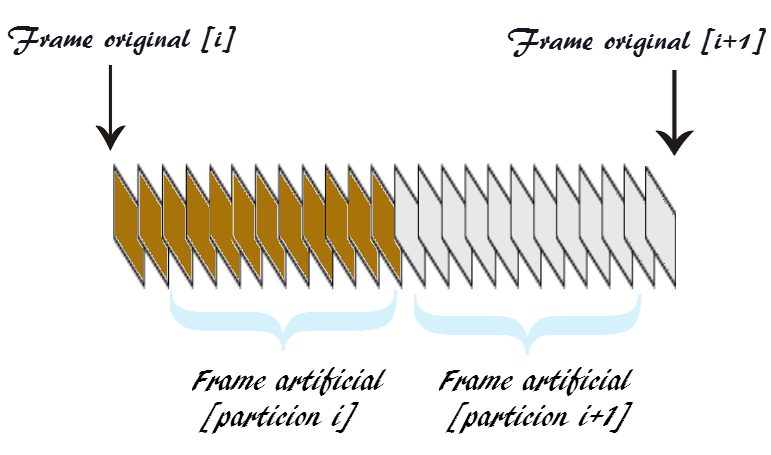
\includegraphics[width=0.55\textwidth]{VecinoCercano.png}
     \caption{Ejemplo de vecino m\'as cercano}\label{fig:vecino}
\end{figure}
\noindent

En el caso de la figura, el par\'ametro de cantidad de cuadros a agregar es de $fr = 22$. Por ende, se lo divide en dos particiones de $11$ frames artificiales cuya imagen corresponder\'a al frame original m\'as cercano (el marr\'on o blanco). Como observaci\'on trivial, el frame original $i$ se lo considera como la imagen reproducida en el estado de tiempo anterior a los artificiales agregados de por medio. An\'alogamente, ocurre con el otro cuadro en el extremo derecho.

Volviendo al an\'alisis del video en su mera totalidad, se repite el anterior procedimiento en cada par de frames en el orden concebido por la secuencia del video. De tal forma, se obtienen los frames artificiales, consiguiendo una nueva filmaci\'on con el efecto de $slowmotion$ que este m\'etodo propone. 

\subsubsection*{\bf{Perspectiva Matem\'atica:}}

\textbf{¿Qu\'e relaci\'on lleva este m\'etodo con el concepto de interpolar?} No dejaremos esta pregunta de lado, pues estar\'iamos ignorando lo que en la introducci\'on le dimos tanta importancia. Como pequeño recordatorio, en interpolaci\'on se buscamos obtener nuevos puntos del plano en base a los datos ya conocidos. Copiar la im\'agen del extremo m\'as cercano equivale a tomar cada p\'ixel del frame original, o sea los datos conocidos, e insertar estos valores en el frame artificial. De hecho, el frame artificial no es m\'as que un ``punto intermedio'' entre los dos frames originales.

Transladamos esto \'ultimo a t\'erminos matem\'aticos para evitar cualquier ambigüedad al respecto. Por cada p\'ixel, se tiene un polinomio al que denominaremos $S_{i,j}$ cuyo \'indice denota a la posici\'on de la matriz del frame que se esta evaluando. Por otro lado, abreviaremos a $frameOriginal_{p}$ al cuadro que esta en el extremo inferior (hecho pasado) y $frameOriginal_{(p+1)}$ al del extremo superior (hecho futuro). Finalmente, $fr$ que simboliza nuevamente la cantidad de frames a adicionar. Definimos a $S_{i,j}$ como:

\[
S_{i,j}(x) = 
\left\{
    \begin{array}{ll}
        frameOriginal_{p}(i,j) & \mbox{si } x \leq fr/2 \\
        \hspace{0.3cm}     
        frameOriginal_{(p+1)}(i,j) & \mbox{si } x > fr/2
    \end{array}
\right.
\]

Por ende, conseguimos transformar una idea, cuyo fundamento se apartaba de este concepto de interpolaci\'on, a desarrollar una funci\'on partida en dos fragmentos. Ambas particiones, tienen la particularidad de ser funciones constantes \footnote{\url{https://es.wikipedia.org/wiki/Funcion_constante}} a lo largo de su dominio. 

Se concluye al hecho de que debido a su posible discontinuidad (solo puede ser continua si ambas particiones comparten la misma constante), los cambios entre cada fragmento podr\'ian detallar un cambio brusco durante la reproducci\'on del video resultante, si es que entre la matriz del frame original y su sucesora, existe una gran desigualdad n\'umerica. Dicho de otras palabras, si la suma 

\[ \sum_{i = 0}^m \sum_{j = 0}^n ( frameOriginal_{p}(i,j) - frameOriginal_{(p+1)}(i,j) )^2 \]

es elevada, luego se puede confirmar un cambio de frame a frame notorio (salto de escena, por ejemplo) que ratifique lo anteriormente dicho. Aunque no los adelantaremos a un terreno que puede ser tentativo para cierta experimentaci\'on.

\subsubsection{Construcci\'on mediante Interpolaci\'on lineal}

Semejante al \emph{cuadro m\'as cercano}, en el sentido que comparten la ideolog\'ia de trabajar c\'iclicamente con cada par de frames para eventualmente, obtener el video deseado con su respectivo efecto. No obstante, contaremos lo particular y caracter\'istico de este m\'etodo, que puede propocionar ciertas mejoras en el movimiento de objetos durante su filmaci\'on.

\subsubsection*{\bf{Conceptualizaci\'on:}}

Por un lado, no posee la misma intuici\'on que su antecesora, donde la im\'agen de cada frame artificial se basa en copiar alguno de los dos cuadros originales en evaluaci\'on. En cambio, se busca utilizar fundamentos matem\'aticos que ayuden a \emph{predecir y reflejar} lo sucedido entre cada par de frames del video original. 

Nuevamente, nos enfocamos en analizar el algoritmo propuesto para la creaci\'on de los $fr$ frames artificiales que se desean adherir entre cada conjunto de pares. En primer lugar, debemos pensar a cada frame como una matriz de $m$ $x$ $n$ p\'ixeles (dependiendo la resoluci\'on en que se dispone el video), siendo $m$ el largo del cuadro y $n$ el ancho. En segundo lugar, el procedimiento destina a generar un polinomio de grado uno \footnote{ Tambi\'en definida como funci\'on lineal; \url{https://es.wikipedia.org/wiki/Lineal}.} entre ese par de frames originales.

Contamos previamente acerca de la representación de tales cuadros como matrices compuestas por p\'ixeles, y de dichos píxeles como números enteros del 0 a 255.

Dicho esto, el m\'etodo se centra en crear un polinomio interpolador por cada posici\'on del frame cuyos puntos interpolados resultan ser los valores de dicha ubicaci\'on en el par de frames originales que se est\'a trabajando. Por ende, tendremos por cada par de cuadros reales, $m$ $x$ $n$ polinomios de grado uno. De lo anterior nace una nueva duda : ¿C\'omo esto resuelve nuestro problema de crear m\'utiples frames artificiales?

El hecho est\'a en que ahora conocemos los valores intermedios entre los dos cuadros originales y en consecuencia, podemos particionar ese dominio en $p$ partes ($p$ siendo la cantidad de frames que se adiciona en cada par) y finalmente, evaluar el polinomio en los bordes de cada fragmento. Como observaci\'on, este paso lo tendremos que aplicar para cada posici\'on de la matriz modelada.

De misma forma, se realiza la tarea sobre cada par agrupado en el orden indicado con lo que eventualmente, el m\'etodo en cuesti\'on concluye con su labor, dejando el efecto de $slowmotion$ que la misma ofrece.

\begin{figure}[h!]
  \centering
    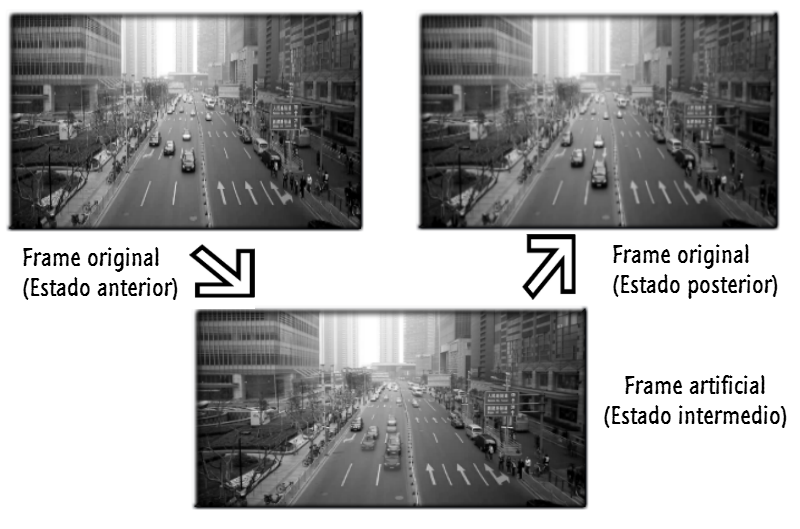
\includegraphics[width=0.65\textwidth]{InterpolacionLineal.png}
     \caption{Muestra de interpolaci\'on lineal con un solo frame intermedio}\label{fig:vecino}
\end{figure}
\noindent

\subsubsection*{\bf{Perspectiva Matem\'atica:}}

Repasamos r\'apidamente lo que en la introducci\'on te\'orica hab\'iamos señalado, aplic\'andolo a la asignaci\'on en cuesti\'on. Construimos $S_0, \ldots, S_{n - 1}$ polinomios tal que $S_i$ interpola $x_i$ y $x_{i + 1}$. Luego, definimos la siguiente funci\'on que adjunta \'estos \'ultimos:
 
\[
f(x) = 
\left\{
    \begin{array}{ll}
        S_0(x)  & \mbox{si } x \in [x_{0}, x_1] \\
        \hspace{0.3cm}\vdots \\     
        S_{n - 1}(x) & \mbox{si } x \in [x_{n - 1}, x_n]
    \end{array}
\right.
\]

Deciframos lo anterior como los polinomios $S_{(i,j)}$, donde el par $(i,j)$ representa a una posici\'on de la matriz frame. Nuevamente, estamos realizando una funci\'on a partir de un par de frames originales tal que el $frameOriginal_{p}$ se figura como el estado anterior y $frameOriginal_{(p+1)}$ el posterior. Aqu\'i yace una diferencia con el m\'etodo del vecino m\'as cercano y es que cada $S_{(i,j)}$ corresponde a una funci\'on lineal. Pasamos a definir a \'esta misma como la siguiente recta:

\[
S_{(i,j)}(x) = y0 + (y1 - y0) * ( ( x - x0 ) / (x1 - x0) ) 
\]

Donde $y0 = frameOriginal_{p}(i,j)$ y $y1 = frameOriginal_{(p+1)}(i,j)$. Por parte de $x0$ y $x1$, lo enumeramos como $0$ y $1$ respectivamente. No importa el valor de estos \'ultimos, mientras sean consecutivos.\footnote{ a x1 = x0 + 1} No obstante, es importante aclarar que siempre se evaluar\'a esta funci\'on dentro del rango $[x0 ,x1]$, es decir, los puntos intermedios.

Para una mayor comprensi\'on, representaremos gr\'aficamente el siguiente ejemplo: Supongamos que tenemos el algoritmo que realiza cada funci\'on $S_{(i,j)}$, recogiendo cada par p\'ixel de igual posici\'on en los dos frames originales escogidos. Notamos que est\'a operando sobre la posici\'on $(1,2)$ y decidimos visualizar dicho resultado. Asumiendo que el par\'ametro $fr = 2$, observamos lo siguiente:

\begin{figure}[h!]
  \centering
    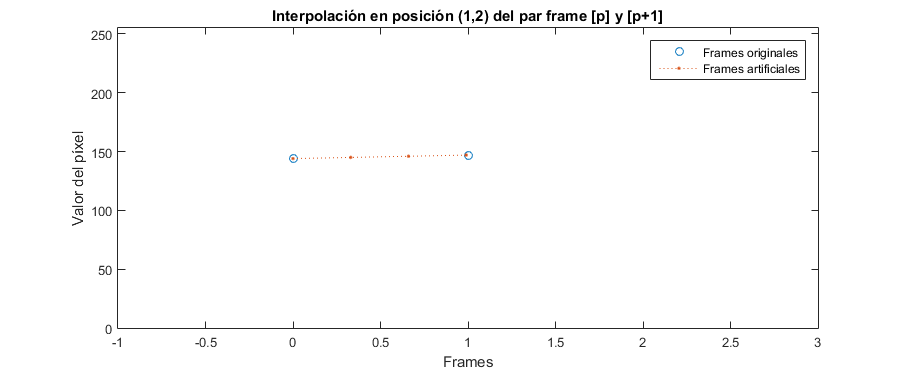
\includegraphics[width=0.85\textwidth]{InterpolacionSimple.png}
     \label{fig:intSimple}
\end{figure}
\noindent

Y as\'i este algoritmo proseguir\'a con su trabajo, hasta llegar al \'ultimo par de frames originales a interpolar. En consecuencia, obtiene la funci\'on explayada al inicio de esta perspectiva matem\'atica.


\begin{figure}[h!]
  \centering
    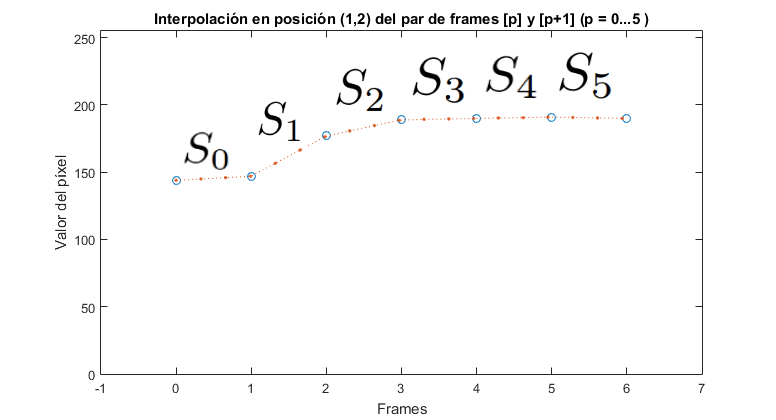
\includegraphics[width=0.75\textwidth]{InterpolacionConjunta.png}
     \caption{Resultado luego de haber interpolado por separado cada $S_{i}$ (con $i = 0 \ldots 5$)}\label{fig:intConjunta}
\end{figure}
\noindent

\subsubsection{Construcción mediante interpolación por splines}

Un m\'etodo que revive con la misma idea de conseguir los frames artificiales o intermedios mediante la evaluaci\'on de cierto polinomio en un determinado punto, pero esta vez aferr\'andose a una mayor complejidad. Sin lugar a dudas, su desarrollo dar\'a la sensaci\'on de brindar resultados m\'as satisfactorios en la construcci\'on del $slowmotion$, aunque habr\'a tiempo para confirmar esto \'ultimo durnate experimentaci\'on y/o conclusi\'on de este informe.